\documentclass[../main.tex]{subfiles}
\begin{document}

\section{SLT}
\subsection{Structural Risk Minimization (SRM) \& VC-dimension}
The feasibility of supervised learning depends on the following key question:\\
Does a training sample consisting of $N$ independent and identically distributed examples
$$(\bold{x}_1,d_1),(\bold{x}_2,d_2),...,(\bold{x}_N,d_N)$$
contain sufficient information to construct a learning machine capable of good generalization performance?\\
The answer to this fundamental question lies in the method of \emph{structural risk minimization}, described by Vapnik (1982, 1998).\\

\noindent Here we consider a second measure of the complexity of $H$, called the Vapnik-Chervonenkis dimension of $H$ (VC dimension, or $VC(H)$, for short). As we shall see, we can state bounds on sample complexity that use $VC(H)$ rather than $\mid H \mid$. These bounds allow us to characterize the sample complexity of many infinite hypothesis spaces, and can be shown to be fairly tight.\\

\noindent $\blacksquare$ \textbf{Shattering \& VC-dim}\\
The VC dimension measures the complexity of the hypothesis space $H$, not by the
number of distinct hypotheses $\mid H \mid$, but instead by the number of distinct instances from X that can be completely discriminated using $H$. To make this notion more precise, we first define the notion of shattering a set of instances.\\ 

\noindent Given $X$ (instance space), $H$ (hypothesis space) and a binary classification, there are $2^N$ possible \textbf{dichotomies} (partitions or labeling of the $N$ points by –1 or +1). A particular dichotomy is \textbf{represented} in $H$ if there exists a hypothesis $h$ in $H$ that realizes the dichotomy.\\

\noindent \textbf{Def:} \emph{H shatters $X$ iff $H$ can represent all the possible dichotomies on $X$ (0 errors)}.
\begin{itemize}
    \item the points in $X$ can be separated by an $h$ in $H$ in all the possible way
    \item for every possible dichotomy of $X$, there exists a consistent hypothesis $h$ in $H$
\end{itemize}
\textbf{Example:}
\begin{figure}[H]
    \centering
    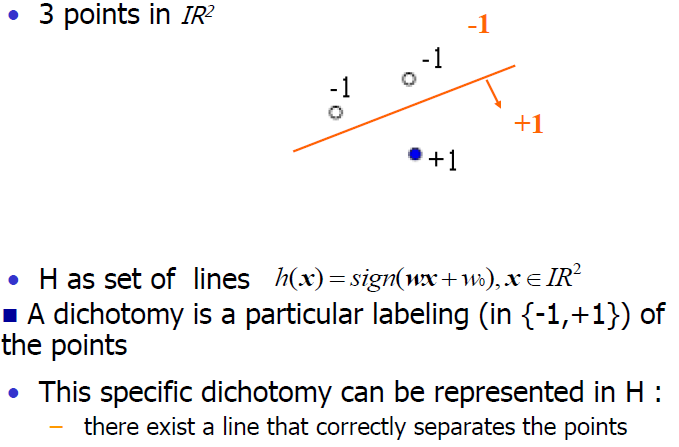
\includegraphics[scale = 0.5]{lectures/5_validation/5_dic_1.png}
\end{figure}
\begin{figure}[H]
    \centering
    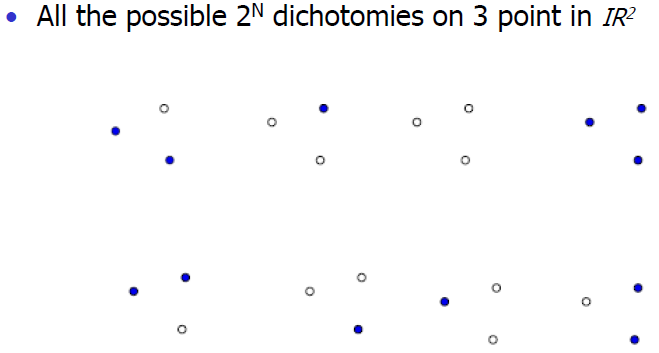
\includegraphics[scale = 0.5]{lectures/5_validation/5_dic_2.png}
\end{figure}
\begin{figure}[H]
    \centering
    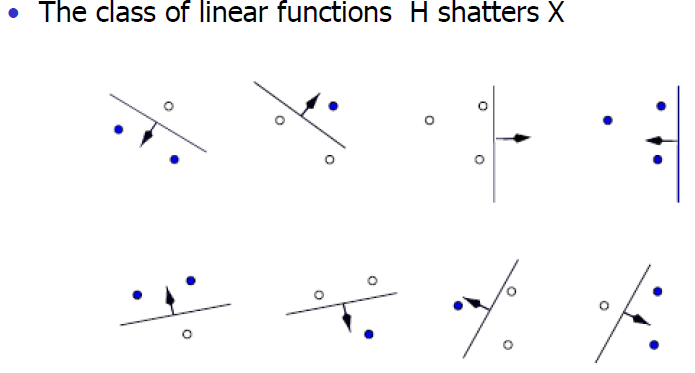
\includegraphics[scale = 0.5]{lectures/5_validation/5_dic_3.png}
\end{figure}
\noindent The ability to shatter a set of instances is closely related to the inductive bias of a hypothesis space. Recall that an unbiased hypothesis space is one capable of representing every possible concept (dichotomy) definable over the instance space $X$. Put briefly, an unbiased hypothesis space $H$ is one that shatters the instance space $X$. What if $H$ cannot shatter $X$, but can shatter some large subset $S$ of $X$? Intuitively, it seems reasonable to say that the larger the subset of $X$ that can be shattered, the more expressive $H$. The VC dimension of H is precisely this measure.\\

\noindent \textbf{Def:} \emph{The \textbf{VC dimension} of a class of functions $H$ is the maximum cardinality of a set (configuration) of points in $X$ that can be shattered by $H$}.\\

\noindent$VC(H)=p$
\begin{itemize}
    \item $H$ \emph{shatters} at least one set (configuration) of $p$ points
    \item $H$ \emph{cannot shatter} any set (configuration) of $p + 1$ points
\end{itemize}
If arbitrarily large (but finite) sets of $X$ can be shattered by $H$, then VC is infinite.\\

\noindent Note that however not all the possible configuration of $N$ (in the example $N=3$) points can be shattered. But it is sufficient to find one configuration of $N$ points which is separable for every labeling.
\begin{figure}[H]
    \centering
    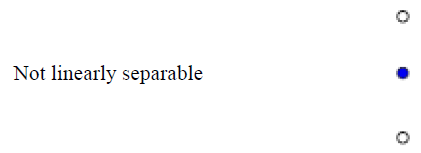
\includegraphics[scale = 0.4]{lectures/5_validation/5_dic_4.png}
\end{figure}
\noindent In general the VC dimension of a class of linear (separator/decision) hyperplanes (LTU) in a \textbf{n}-dimensional space is \textbf{n+1}.\\

so the VC-dim of a linear function is:
\begin{figure}[H]
    \centering
    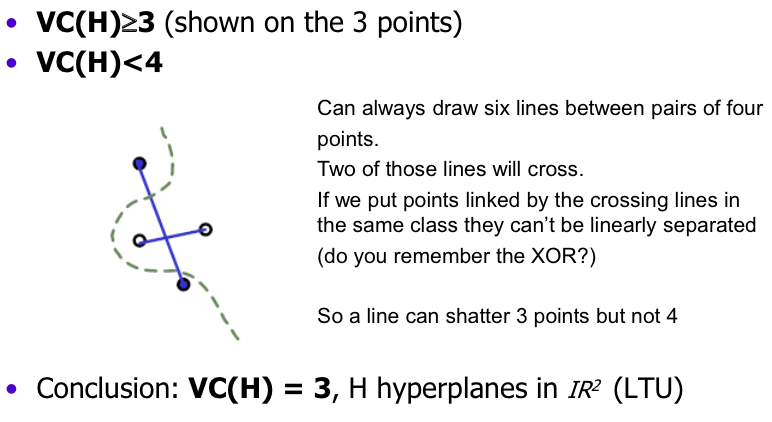
\includegraphics[scale = 0.4]{lectures/6_SLT/vc_linear_f.png}
\end{figure}
\noindent $\blacksquare$ \textbf{Number of parameters and VC-Dim}
Is VC the number of parameters? It can be related but not really the same:
\begin{itemize}
    \item Of course, we may add redundant free parameters
    \item there exist models with one parameter and infinite VC dim
\end{itemize}
Moreover, for nearest neighbor VC-dim is infinite: The VC dimension of a 1-nearest-neighbor classifier is infinite. Given any set of points, it will correctly classify 100\% of those points since each point is the closest point to itself. In this case the number of parameters in the k-nn is infinite, because is infinite the number of patterns (N) and the number of parameters is given by N/k. Infact, with $K=1$ we have overfitting with K-nn and the error is really high and the VC-dim is very high.\\

In neural networks the number of units (so more weights to the net) can give an high complexity and an high VC-dim.\\

\noindent\textbf{Other Note on K-NN and VC-Dim}\\
At first glance, k-nearest neighbors has a single parameter, that is k, the number of neighbours to be included in deciding on the majority-vote predicted classification.

However, the effective number of parameters to be fit is not really k but more like n/k. This is because the approach effectively divides the region spanned by the training set into approximately n/k parts and where each part is governed by the majority vote classifier.

To form an analogy with a parameterised model (e.g. GLM) if you have a dataset of size n 50, a choice of k=25 for kNN results in an effec­tive number of parameters of about 2 and is comparable in the extent of smoothing / degree of freedom to a linear regression fit with two coefficients.

P.S. For kNN, the effective number of parameters / the degree of complexity is known as Vapnik–Chervonenkis (VC) dimension.\\

\noindent $\blacksquare$ \textbf{SLT: Analytical Bound on R}
\begin{figure}[H]
    \centering
    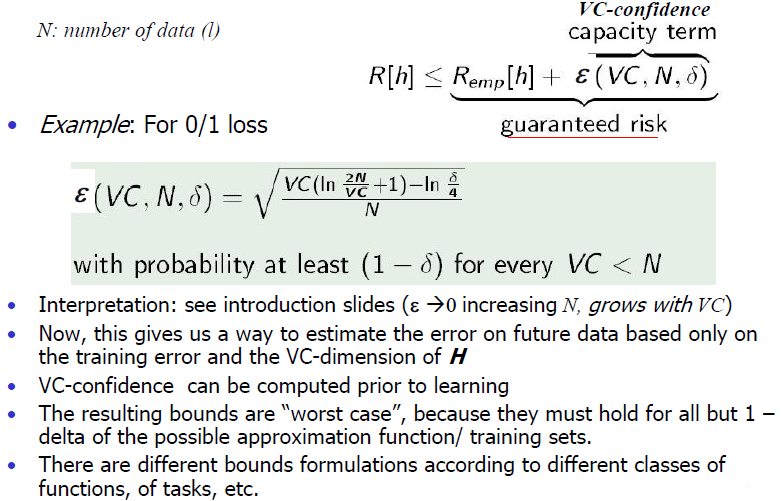
\includegraphics[scale = 0.6]{lectures/5_validation/5_slt.png}
\end{figure}
Example of consequences:
\begin{itemize}
    \item For many reasonable hypothesis classes (e.g., linear approximators) the VC dimension is linear in the number of “parameters” of the hypothesis.
    \item This shows that to learn “well”, we need a number of examples that is linear in the VC dimension (so linear in the number of parameters, in this case).
\end{itemize}

\noindent $\blacksquare$ \textbf{Structural Risk Minimization}\\
\noindent SRM uses VC dimension as a controlling parameter for minimizing the generalization bound on R. Assuming finite VC we can define a nested structure of models- hypothesis spaces according to the VC-dim as in the following
$$H_1\subseteq H_2 \subseteq ... \subseteq H_n$$
$$VC(H_1)\leq VC(H_2) \leq ... \leq VC(H_n)$$
In effect,the size of $H_n$ is a measure of the machine capacity.\\

\noindent $\blacksquare$ \textbf{SRM for model selection}
\begin{figure}[H]
    \centering
    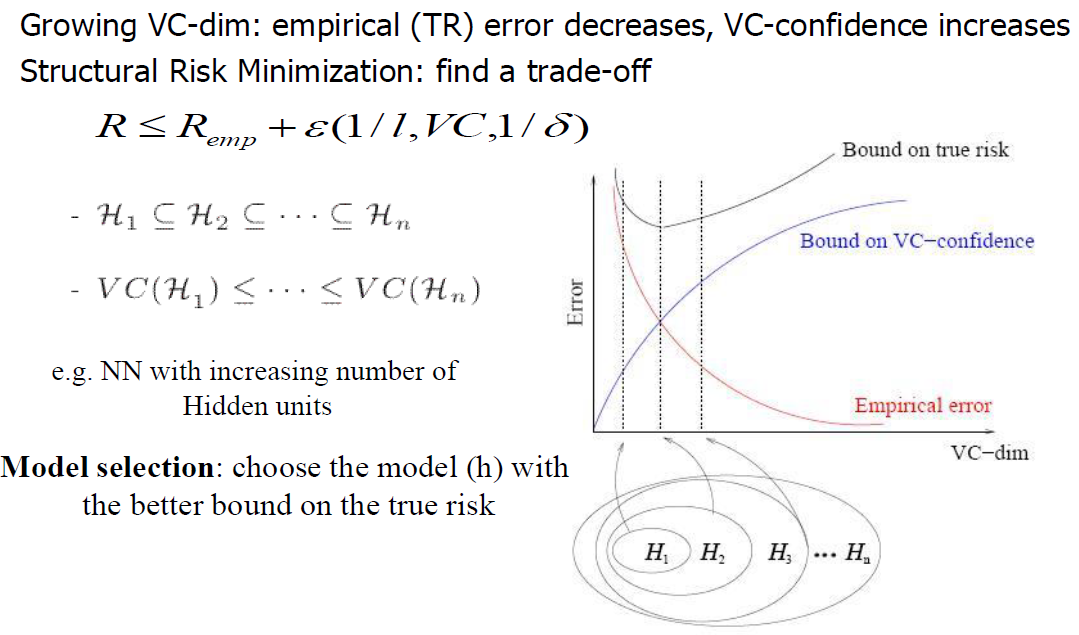
\includegraphics[scale = 0.5]{lectures/5_validation/5_srm_model.png}
\end{figure}
\noindent This doesn't work in practice, infact the VC-Conf can result very conservative: hundreds of times larger than the empirical overfitting effect.\\

\noindent $\blacksquare$ \textbf{SRM Approaches}
$$R \leq R_{emp} + \epsilon(1/l,\,VC,\,1/\delta)_{VC-confidence}$$
For instance two practical approaches
\begin{itemize}
    \item Choose appropriate structure/complexity, fix the model (and hence the VC-confidence), minimize TR error (e.g. can be used in NN)
    \begin{itemize}
        \item However regularization due to training heuristic can further introduce a implicit SRM implementation (early stopping, …)
    \end{itemize}
    \item Fix the TR error, automatically minimize the VC-confidence: how ? We will see.
\end{itemize}

\end{document}